Většinu chemiků zajímá dění v~základním elektronovém stavu: jaká je struktura molekul, kapalin, či krystalů, jaké jsou solvatační či mřížkové energie, jaké je rovnovážné složení reakční směsi atp. S~elektronově excitovanými stavy se nicméně chemik setká v~souvislosti s~různými spektroskopickými technikami: UV absorpční spektroskopie, rentgenová spektroskopie, spektroskopie založené na elektronovém cirkulárním dichroismu či v~nejrůznějších fluorescenčních technikách. Nesmíme přitom zapomenout ani na samostatné odvětví chemie zaměřené na chemii světla, na fotochemii. Porozumět vlastnostem elektronově excitovaných stavů je důležité v~nejrůznějších aplikacích, od biofyzikálních problémů (Jak probíhá fotosyntéza? Jakým  způsobem je přenášen zrakový vjem) až po technologie a materiálové inženýrství (Jak fungují solární články?). 

Na první pohled se zdá, že není nutné pro excitované stavy vytvářet samostatný oddíl. Jestliže řešíme elektronovou Schr\"odingerovu rovnici

\begin{equation}
\hat{H} \psi_i = E_i \psi_i
\label{rov:Ex-1}
\end{equation}

\noindent získáváme tak kromě energie základního stavu $E_0$ a příslušné vlnové funkce $\psi_0$ i stavy excitované s~energiemi $E_i$, $i > 0$. Tak tomu v~principu je, nicméně je třeba mít na paměti, že většina kvantově-chemických metod, které byly doposud v~našem textu představeny jsou designovány pro výpočty v~základním elektronovém stavu a jejich použití pro excitované stavy bez dalších úprav není možné. Příkladem mohou být metody založené na teorii funkcionálu hustoty. Hohenbergovy-Kohnovy teorémy jsou odvozeny pro elektronovou hustotu základního stavu a~rozšíření metody DFT do excitovaného stavu není vůbec samozřejmé. Při výpočtech excitovaných stavů musíme být také ostražití při volbě jednoelektronové báze. Zatímco v~základním stavu se vlnová funkce typicky příliš nevzdaluje od atomových jader, ve stavech vzbuzených může být úplně jinak.  

Příkladem metod, které je snadné rozšířit do excitovaného stavu, jsou přístupy založené na metodě konfigurační interakce. Zejména vhodné a často používané jsou multireferenční přístupy (viz kapitola \ref{kap:abinitio}). Často se tak setkáme s~metodou CASSCF a jejich poruchovým  vylepšením CASPT2 či s~vylepšením pomocí metody konfigurační interakce, metodou MRCI.   

Předpokládejme nyní, že jsme schopni vypočítat energie a vlnové funkce základního i excitovaného stavu. Mohlo by nás zajímat, kdy pak bude světlo o~frekvenci $\nu$ absorbováno či kdy naopak molekula ve vzbuzeném stavu přeskočí do stavu základního za vyzáření fotonu o~energii $h\nu$. Musí být především splněna rezonanční podmínka 


\begin{equation}
h \nu = E_j - E_i,
\label{rov:Ex-2}
\end{equation}

\noindent která nám řekne, jaké fotony budou absorbovány nebo emitovány. Kromě toho by nás ale mělo také zajímat, jak intenzivní příslušná absorpce či emise světla bude. To se dozvíme prostřednictvím veličiny nazvané \textbf{tranzitní dipólový moment}


\begin{equation}
\vec{\mu}_{ij} = \int \psi_i^{\ast} \vec{\mu} \psi_j \mathrm{d} \tau,
\label{rov:Ex-3}
\end{equation}


\noindent kde $\vec{\mu}$ je dipólový moment pro dané okamžité uspořádání elektronů a atomových jader, $\psi_i$ je vlnová funkce počátečního stavu, $\psi_j$ je vlnová funkce konečného stavu. Z~experimentálního hlediska je intenzita absorpce charakterizována molárním absorpčním koeficientem $\epsilon$, který vystupuje v~Lambertově-Beerově zákonu

\begin{equation}
I = I_0 \cdot 10^{-\epsilon c l},
\label{rov:Ex-4}
\end{equation}

\noindent kdy $I_0$ je intenzita záření vstupujícího do kyvety, $I$ je intenzita světla vystupujícího, $l$ je délka kyvety a $c$ je koncentrace absorbujících částic. S~využitím časově-závislé Schr\"odingerovy rovnice se dá ukázat, že molární absorpční koeficient je přímo úměrný druhé mocnině tranzitního dipólového momentu

\begin{equation}
\epsilon \sim \vert \vec{\mu}_{ij} \vert^2.
\label{rov:Ex-5}
\end{equation}

Tranzitní dipólový moment tak představuje ústřední veličinu v~teoretické spektroskopii. Na základě analýzy výrazu \eqref{rov:Ex-5} se odvozují tzv. \textbf{výběrová pravidla}, která nám říkají, které z~přechodů jsou dovolené a které z~přechodů jsou naopak zakázané.

Absorpční a emisní spektra atomů jsou nesmírně úzká, v~podstatě čárová. stejně tak spektra odpovídající rotačním či vibračním přechodům nejsou příliš široká. To je dáno nutností splnit rezonanční podmínku \eqref{rov:Ex-3}. Naproti tomu absorpční a fluorescenční spektra molekul jsou často velmi široká, s~šířkou o~desítkách nanometrů. Toto rozšíření spektrálních čar je dáno vibracemi molekul v~základním stavu (tedy pohyby nulových kmitů). Celý koncept je demonstrován na obrázku~\ref{obr:Absorpce}: molekula vibruje  a my ji tak s~různou pravděpodobností nacházíme v~různých geometriích. Každé geometrii přitom odpovídá jiná rezonanční podmínka. Absorbujeme proto fotony o~různých vlnových délkách.

\begin{figure} [htb]
\centering
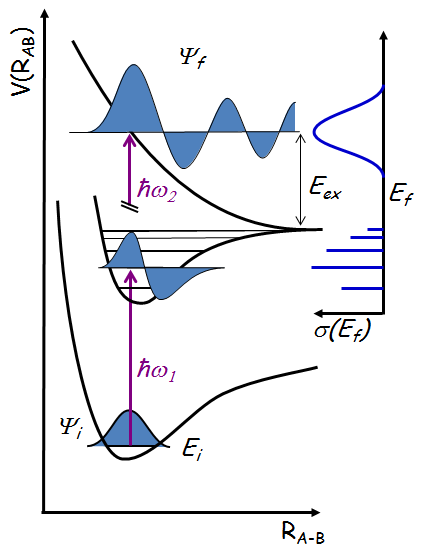
\includegraphics[scale=0.5]{Absorpce.png}
\caption{Absorpční spektrum molekul.}
\label{obr:Absorpce}
\end{figure}

Existuje ještě jedna cesta umožnující vypočítat energie excitovaných stavů a intenzitu absorpce, aniž bychom přitom ale znali vlnovou funkci excitovaného stavu. V~kapitole \ref{kap:vlastnosti} jsme diskutovali veličinu nazvanou polarizovatelnost. Ta nám říká, jak moc je molekula citlivá na vnější elektrické pole. Vnější elektrické pole může být ale i časově proměnné, v~případě světla o~frekvenci $\nu$ se intenzita elektrického pole mění harmonicky dle vztahu

\begin{equation}
\vec{E}(t) = \vec{E_0} \sin (2 \pi \nu t).
\label{rov:Ex-6}
\end{equation}

Můžeme se nyní tázat, jak je molekula citlivá na elektrické pole o~této frekvenci. Získáme tak frekvenčně závislou polarizovatelnost molekuly $\alpha(\nu)$. Tato veličina prudce vzrůstá v~okamžiku, kdy je splněna rezonanční podmínka \eqref{rov:Ex-3}. V~principu tedy potřebujeme simulovat zkoumanou molekulu umístěnou do časově-proměnného pole, což vlastně odpovídá experimentu. K~tomu je potřeba časově-závislá Schr\"odingerova rovnice. V~praxi je možné pro málo intenzivní pole nutnost použití časově závislé Schr\"odingerovy rovnice obejít. Na tomto principu jsou založeny metody jako je velmi efektivní \textbf{metoda časově-závislé teorie funkcionálu hustoty} TD-DFT (z~angl. \textit{Time Dependent Density Functional Theory}), představující rozšíření DFT metod do oblasti excitovaných stavů nebo kupříkladu metoda EOM-CCSD (a angl. \textit{Equation of Motion Coupled Clusters Single and Double excitations}), což je zase rozšířením metody spřažených klastrů do oblasti excitovaných stavů. 
   

 

           
      

   




 




      

      



